In this section we first identify solutions similar to TABuss, found in Trondheim and in other parts of the world, before we describe the development process.

At the beginning of the project, MultiBRIS\cite{multibris} planned the implementation of a server hosting the application logic, including the communication with BusTUC\cite{busstuc} and AtB's real-time system. The development sections first describe the implementation of TABuss without thinking about the server functionalities. Then, the shifting to the server and necessary adjustments are described.


\subsection{Raaum's BusTUC Android Application}

BusTUC Android Application is the application that was created by Magnus Raaum\cite{mag}. It displays a map with user and bus stop locations, and an input field for entering the desired destinations. The system uses the closest bus stops to a user's location to search for possible routes, by sending queries to BusTUC. Received departure suggestions are then updated with real-time departure times, before they are shown to the user as plain text suggestions.

\subsection{Existing Solutions in Trondheim}
\label{sec:existingtrondheim}
The following sections describe existing applications, developed for getting info about bus transportation in Trondheim. 
\begin{table}[!h]
\label{tab:funcintest}
\begin{center}
   \caption{Functionality in the tested applications.}
    \begin{tabular}{ |  l  |  l  |  l  |  l  |  l  |  }
    \hline
    Application & Bartebuss & Alf's Bybuss & Bussdroid & Busstider\\ \hline
    Bus oracle & Yes & Yes & Yes & Yes \\ \hline
    Map & Yes  & Yes & No & Yes \\ \hline
    Favourites & Yes & No & No & No \\ \hline
    History & Yes & Yes & Yes & No \\ \hline
    Real-time & Yes & Yes & Yes & No \\ \hline
    \end{tabular}
\end{center}
\end{table}
Table \ref{tab:funcintest} gives a summarised comparison of the tested applications. Below a brief description of each criteria is given. The following sections describe all the tested applications.
\\\\
\newpage
\begin{description}
\item [BusTUC]
Whether the tested application uses BusTUC as a functionality
\item [Map]
Whether the tested application integrate maps
\item [Favourites]
Favourites functionality allows a user to store queries or specific bus stops for later use. A typical usage is to store a query with an additional tag
\item [History]
History defines earlier searched queries or selected bus stops, stored in the internal or the external storage
\item [Real-time]
Whether the tested applications provide real-time data.
\end{description}

\subsubsection{Bartebuss}
\label{sec:bartebuss}
\emph{Bartebuss}\footnote{http://bartebuss.no/om} is developed in HTML5 by Rune M. Andersen,  and uses the \emph{BusBuddy} API\footnote{http://busbuddy.norrs.no/}. It has rich functionality, with options to store favourites, find near-by bus stops, search for specific bus stops, use BusTUC and show maps. Due to the use of HTML5, the map is not as responsive as in a native application. The user interface on the other hand is intuitive and easy to navigate but it might provide too many choices to the user.
\setlength{\intextsep}{0pt}
\begin{wrapfigure}{l}{0.5\textwidth}
  \begin{center}
    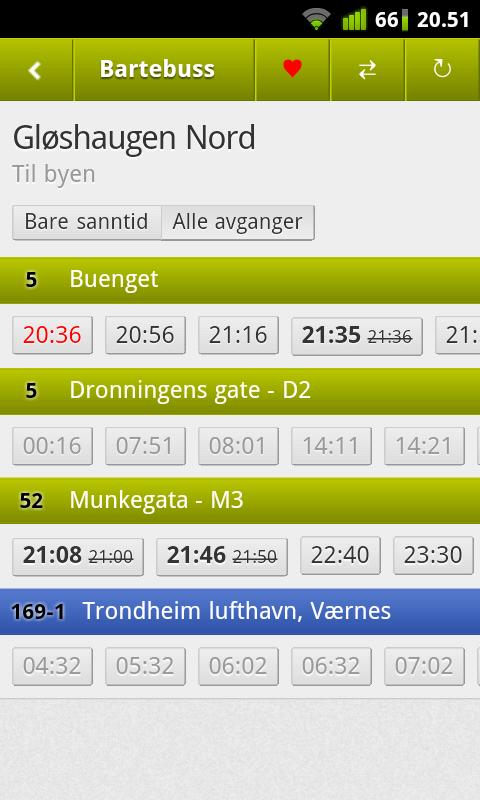
\includegraphics[scale=0.25]{ExistingSolutions/bartebuss.jpg}
  \end{center}
  \caption{Bartebuss}
\end{wrapfigure}
\setlength{\intextsep}{3pt}
There are 5 ways to use the application to find bus departures. The first is through ''favourites'', where several bus stops can be stored(giving quick access). When a favourite is selected, real-time data for the bus stop is displayed. The second way to use the application is an option called ''near me'', where the closest bus stops to a user's location are listed. Items can be selected the same way as in favourites. The third option is ''search''. Here, the user can search for a specific bus stop, and view real-time data. The fourth option is BusTUC, where a text field is used for query input. The last option is to select a bus stop icon from the map, which triggers a rewrite of real-time data. The map part was lagging during testing on the Android platform, and hardly usable at all. Two other problems are the lack of pinch zooming and poor handling of landscape/portrait changes(as resizing causes problems). When tilted to landscape mode, the zoom controls disappear.

\subsubsection{Alf's ByBuss}
\emph{Alf's ByBuss} \footnote{http://bybuss.alfsimen.com} is a native Android application, developed by Alf Simen S\o rensen. It also uses the \emph{BusBuddy} API. It has a simple user interface, and provides BusTUC functionality, with the option to include the user's location as the departure parameter.
The application has a text field for entering queries, and some additional functionalities in the menu (activated by the menu button). The main component of the user interface is a map showing clickable bus stop icons. The user can select the bus stop icons, with corresponding bus stop names, as departure and destination, and view real-time data. Menu options include: ''Use my existing location''(which inserts the user's current location into the text field as departure input), ''reverse search''(which switches the departure and destination stops), and a link to the online bus schedules. \emph{Alf's ByBuss} appears more responsive than \emph{Bartebuss} during map navigation, but the user interface is not as polished. 
\subsubsection{Bussdroid}
\emph{Bussdroid} \footnote{market.android.com/details?id=com.ken.bussdroid} is a native Android application by Ken B\o rge Viktil. Unlike the two previously tested applications, it does not provide a map. The functionality consists of real-time data for bus stops, a BusTUC query text field and the possibility to store queries as favourites. The application is responsive, and has a clean and intuitive user interface. 

\subsubsection{Busstider}
\emph{Busstider} \footnote{http://www.a2bsoft.net/projects/busstider} is a native Android application by Martin M. Syvertsen. Functionality is limited to BusTUC, and a map displaying bus stop icons. Real-time data is not available. There are two ways to use the application: 1) Asking BusTUC with a natural language query, 2) selecting departure and destination by clicking icons on the map. It has a simple and intuitive user interface based on tabs, and is fairly responsive.
\begin{figure}[!h]
\begin{tabular}{ccc}
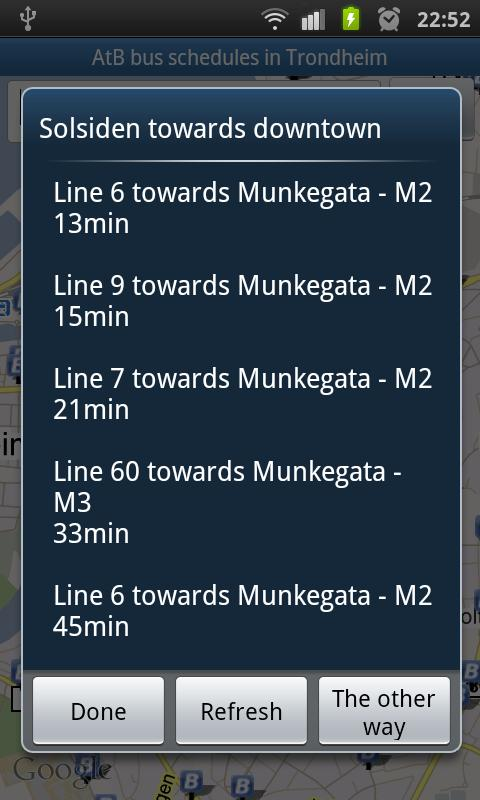
\includegraphics[width=0.27\linewidth]{ExistingSolutions/alfsbybuss.jpg} & 
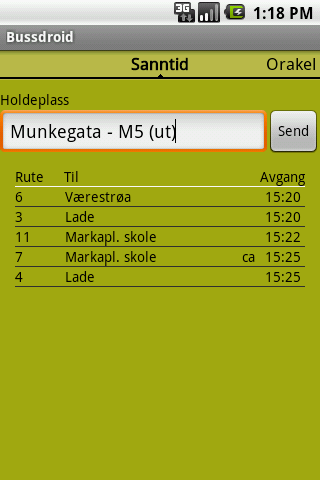
\includegraphics[width=0.27\linewidth]{ExistingSolutions/bussdroid.png} &
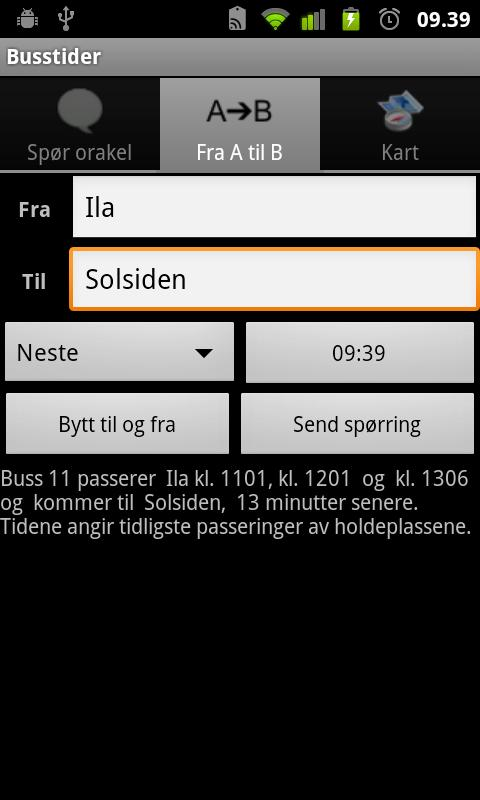
\includegraphics[width=0.27\linewidth]{ExistingSolutions/busstider.jpg}\\
\end{tabular}
\caption{From left to right: (1)Alf's ByBuss, (2)Bussdroid, (3)Busstider}
\end{figure}
\newpage
\subsubsection{BusBuddy API}
\emph{BusBuddy}\footnote{http://api.busbuddy.no/} is an API developed by Roy Sindre Norangshol, aimed at the retrieval of real-time data. It is a hobby project with the goal to minimise the overhead of SOAP messages downloaded to the mobile devices. Both \emph{Bartebuss} and \emph{Alf's ByBuss}, use this API. All applications developed with the \emph{BusBuddy} API are available through GIT Hub\footnote{https://github.com/}, as \emph{BusBuddy}'s policy is that development projects should be open source. 

In the early stages of the project using this API was considered . However, the disadvantages lead to discarding of the idea. As it is a hobby project, retrieving a license key was not easy. In addition, \emph{BusBuddy}'s username and password for access to AtB's real-time system is not permanent. AtB can retract this at any time. The process of retrieving new keys, would have to go through the \emph{BusBuddy} crew. By using the username and password provided by LingIT, this ``middle man'' operation is avoided. It is also likely that AtB would renew the username and password quicker for LingIT, than for a private operator.

\subsubsection{Summary of Existing Solutions in Trondheim}
All the tested applications for bus route information in Trondheim are already downloaded by several users, indicating that they have attractive functionalities. For our project it was important to investigate what has to be done to move the concept of a bus route information application to a new level. And also to compare the different levels of artificial intelligence in the apps. 

Especially \emph{Alf's ByBuss} and \emph{Bartebuss} are close to our goals: they use BusTUC, maps and real-time functionality. Both \emph{Alf's Bybuss} and \emph{Bartebuss} integrate natural language through BusTUC, but aside from this, they do not have any other functionalities involving artificial intelligence. Their functionalities are based only on user input and menu navigations. The main topic of our project is reducing user input. In Raaum's application, route suggestions were calculated based on the closest stops to the user's location, and were automatically updated with real-time departure times. This is the core of the development of TABuss. Though the display of real-time data when a user presses a bus stop icon is an important functionality, we have to keep in mind the artificial intelligence aspects. This can separate our project from \emph{Alf's ByBuss} and \emph{Bartebuss}, and give us an upper hand regarding market potential.

\subsection{Extended Research}
Even though there are several applications available in Trondheim for bus route information, an expanded view including other cities and research performed is more informing. As discussed in Section \ref{sec:existingtrondheim}, aside from the general use of BusTUC, no functionalities in the tested applications can contribute to moving TABuss forward in the field of artificial intelligence. This section describes research areas within bus route information systems, with the main focus on intelligence through natural language, and the use of real-time data. 

\subsubsection{Natural Language Applications}
In intelligent route information systems, natural language has been addressed by different reseach papers\cite{Raux03let'sgo:}\cite{Turunen_mobilespeech-based}\cite {Turunen_designof}\cite{Turunen06evaluationof}. 

Raux et al.(2003) developed a system called \emph{Let's go}, which uses speech through phone calls as input, for returning route information\cite{Raux03let'sgo:}. The system was developed for ''elderly and non-native English speakers'', and provided information for the city of Pittsburgh. Speech was recognised by comparison and retrieval of the closest match. Emphasis was on creation of a grammar model for spoken language, and to include an overall generality regarding different structuring of sentences with the same meaning. Through their work, Raux et al. identified several challenges with speech processing and route information. The main challenge was that different users structured the same phrases differently, when referring to bus stops or places. Hypothetically, assuming BusTUC has a similar up to date speech system (\emph{TeleBuster}\footnote{http://www.idi.ntnu.no/~tagore/telebuster/} is not in use), this system would have to be able to infer correct mappings from spoken text, and also be able to extract content from text spoken with different dialects. As Trondheim is a city with inhabitants from different areas of Norway, this could become a complex operation. 

Turunen et al. (2007)\cite{Turunen_designof} (2006)\cite{Turunen06evaluationof} proposed a similar solution, \emph{TravelMan}, developed for the city Tampere in Finland. \emph{TravelMan} is an updated version of \emph{StopMan}\cite{Turunen_mobilespeech-based}(2006), which provided route planning. Input consisted of locations or addresses, provided to the system by text or speech. The user could also set personal preferences, such as exclusion of transportation options, as \emph{TravelMan} in addition to bus transportation, covered metro and tram. Of other features, a guidance functionality for visually impaired users was implemented, to provide what was referred to as an ''unbroken trip chain''. An unbroken trip chain was a successful trip, completed with full system guidance.


An interesting feature in \emph{TravelMan} related to our project, is the use of context and user location. The real-time guidance relies on location information, which also could be used to infer departure addresses. 
A video of TravelMan in use is available at YouTube \footnote{http://www.youtube.com/watch?v=bPVAQtHtC3s}

\subsubsection{Real-time Bus Information}
Early research focused on finding an optimal route. The Traveling Salesperson Problem \cite{tsp} is transferrable to route information, and several algorithms have been proposed. An example is Robert J. Szczerba et al.'s (2000) paper, which described an adaptation of the A*\cite{astar} algorithm, for finding the optimal route in real-time\cite{szc}. Assuming bus route companies incorporate a similar feature when planning routes, an algorithm including traffic information could give a real-time estimate of where the bus is at a given time. 

Maclean and Dailey's \emph{MyBus}(2000) predicts real-time arrival of buses by using historical data, the bus schedule and an prediction algorithm\cite{mybus}. This algorithm, based on Kalman filters \cite{kalman}, produced estimates, where traffic and passenger information is used as noise, affecting the original schedule.

Maclean and Dailey also published an article on a \emph{Mobile MyBus}(2001), which used communication through WAP\cite{maclean}. This system gave users real-time information based on received input. The input consisted of destination and a route number, sent by a URL request, and forwarded to the \emph{MyBus} server. Both were provided as digits as devices at that time did not have any input mechanism similar to a computer keyboard. In our project, this functionality can be compared to retrieving a real-time ID for a bus stop, before sending a SOAP-request to fetch real-time data. 

\begin{wrapfigure}{l}{0.5\textwidth}
  \begin{center}
    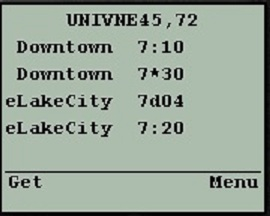
\includegraphics[scale=0.8]{ExistingSolutions/mybus.jpg}
  \end{center}
  \caption{MyBus WAP}
\end{wrapfigure}

Today, buses have GPS-trackers on-board, transmitting location information to a server. Real-time data is updated at specific time intervals and is fairly accurate. The real-time service was introduced in Trondheim by AtB. A similar service is provided in Oslo\footnote{http://trafikanten.no/}.

Ferris, Watkins and Borning's \emph{OneBusAway}(2010)  \footnote{www.onebusaway.org} focuses on context awareness in addition to the use of real-time data\cite{Onebusaway}. \emph{OneBusAway} uses the location of the user to automatically display the closest bus stops on a map, similar to TABuss. Context aware functionality proved to be successful through user testing, where 93 per cent of the existing users of \emph{OneBusAway} reported that more concise information was provided.

What differs \emph{OneBusAway} from TABuss, is that TABuss' main query functionality only needs the users destination as input. \emph{OneBusAway} needs to know both the departure stop and which route to select in order to reach planned destination. 


\subsubsection{Summary of Extended Research}
Both \emph{TravelMan} and \emph{Let's Go} utilise speech recognition to provide route information.\emph{TravelMan} extended the concept even further by introducing real-time guidance based on user location, and had features worth researching for future functionality. It was shown through Turunen et al.'s work that natural language has potential for mobile development and route information applications. 

BusTUC has since its release become a popular choice in Trondheim. As users have become familiar with the usage of natural language, a logical next step could be to introduce speech. iPhone 4S has implemented a system called SIRI\footnote{http://www.apple.com/iphone/features/siri.html}, which also contributes to familiarising people with natural language.

Research on the usage of real-time information has shown progress; from using estimated real-time, to actual real-time data. Maclean and Dailey's \emph{MyBus} WAP version was used over 9000 times, in a time period between its release in September 2000-January 2001, giving an indication that real-time route information on mobile devices is a promising field.


\subsection{Testing}
In this section we identify several existing problems that will be fixed in this project, or in the extension projects in the spring 2012.

\subsubsection{Testing Raaum's Application}
 \label{sec:testing}
Raaum's original source code compiled and ran ''out of the box'', and only required a switch of the API-key, to get the Google Maps integration working. It crashes occasionally, when not reaching the BusTUC server, caused by exceptions that are not caught in the source code. To test the application, several queries were executed, and success rates and response times were monitored. The response times varied between 20 and 40 seconds, which was much slower than the applications reviewed in section \ref{sec:existing}.  It is worth mentioning that the 20-40 seconds monitored for a run includes computations performed with multiple bus stops. A query with one bus stop, took 5-10 seconds to perform on average.


Table \ref{fig:test} displays the time needed to perform five queries, with origin at Gl\o shaugen and destination at Ila. 
\begin{center}
\begin{table}[!h]
\caption{Tested queries.}
\label{fig:test}
\small{
    \begin{tabular}{ |  l  |  l  |  l  |  l  |  l  |  l |}
    \hline
    Run & 1 & 2 & 3 & 4 & 5 \\ \hline
    Time BusTUC & 18 sek & 17 sek & 19 sek & 16 sek & 19 sek \\ \hline
    Time Real-Time & 5 sek & 7 sek & 7 sek & 6 sek & 7 sek \\ \hline
    Time Total & 23 sek & 24 sek & 26 sek & 22 sek & 26 sek \\ \hline
    \end{tabular}
        }
    \end{table}
\end{center} 
The results show that the queries to BusTUC were the most time consuming, while the real-time queries were much quicker.

Slow query runs were caused by the BusTUC server, located at Gl\o shaugen. The other applications tested, used servers hosted by Amazon\footnote{http://aws.amazon.com/ec2/}. The Amazon servers are faster as a result of threading and the use of sockets, performed by a Python script. The server at Gl\o shaugen uses a slower approach with a  PHP-script that runs in the background. This script reads queries from files, and writes queries and results to files. The Prolog side of BusTUC checks these files at given intervals, and processes the queries.

The two different approaches give two different responses: to use the BusTUC hosted by Amazon, only the standard BusTUC syntax(defined in section \ref{sec:bustuc}) can be used, and the results are returned as text. The BusTUC hosted at Gl\o shaugen returns a parseable JSON object, in addition to the text, if the new BusTUC syntax is used. In Raaum's application, the latter format was required for the real-time updates of route suggestions. An uncaught exception was thrown if the returned JSON objects contained errors. As a remark, the returned JSON objects from BusTUC does not follow correct JSON syntax. The JSON objects contain ''<br>'' html-tags, which have to be removed for a parser to be able to recognise the structure. 


To benefit from using the faster Amazon servers, some adjustments have to be made. The servers do not include JSON objects in their results, and a direct swap is not an option as important information is lost when using only the text answers. This JSON information includes bus stop IDs and transfer details. A switch to the Amazon servers would also complicate debugging. Debugging the server at NTNU can be done \emph{white box}, as root access is available. It is unlikely that we would get access to the Amazon servers. 


\begin{wrapfigure}{l}{0.5\textwidth}
  \begin{center}
    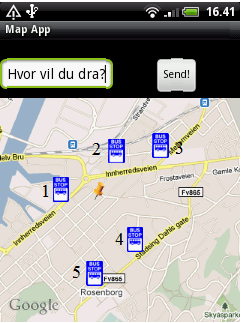
\includegraphics[scale=1]{TestingTheApplication/screen1.png}
  \end{center}
  \caption{Bus stop icons}
\label{fig:icons}
\end{wrapfigure}

Raaum's application uses an XML-file containing: bus stop locations, bus stop names and bus stop IDs, which does not contain sufficient information: information for several bus stops are missing. Also, the list also only contains one bus stop description per ''bus stop group''. A bus stop group consists of one or more bus stops with the same bus stop name. This is a problem in the extraction of real-time data, as a unique bus stop ID is necessary for each bus stop in a bus stop group. Figure \ref{fig:icons} illustrates this problem: only one icon is displayed for each stop group. 

Raaum's application has two sorting errors: one when the total travel time is equal for more than one route suggestion returned by BusTUC, and one when the distances are equal to two or more bus stops from the user's location. The error source is the use of HashMaps\footnote{http://docs.oracle.com/javase/1.4.2/docs/api/java/util/HashMap.html}, with total times or distances from the user's location to bus stops as keys. Keys in HashMaps are unique, because multiple equal keys overwrite the previous mapped value. In the total travel time issue, this leads to an exception as one or more route suggestions are overridden. In the distance issue,the error leads to a wrong display of bus stop icons on the map.

Raaum's application occasionally crashes during parsing of real-time data. This happens because the wrong node is extracted for some numbers. The extracted route numbers sometimes contain the letter ''N'', which in turn causes an exception when parsed as an integer. 

Queries with the new BusTUC syntax were meant to incorporate walking time to a bus stop in minutes. After testing, this was discovered to be ignored in BusTUC's reasoning. Time offsets may assure that unrealistic route suggestions are dropped. But on the other hand, real-time data is only available for bus departures in the ''near future'', and later real-time departure times are equal to the scheduled time. Syntacticly, it is a challenge to add text in the nested query syntax. A working syntax was: \emph{(Samfundet +2) fra Samfundet til Tiller etter $n$}. This was reasoned by BusTUC as if we wanted a bus departure after $n$.
 

Another issue is the handling of transfers, where two or more bus travels are needed to reach a destination. Raaum's application often suggests routes where the transfer bus departs before the first bus has arrived. This happens when the real-time data replaces the scheduled departure times returned from BusTUC, and no further sanity checks are performed. Although this does not cause an exception, the returned answers are unintelligent. 

The application crashes every time \emph{Lade} or \emph{Ranheim} is entered as input, while \emph{Lademoen} and \emph{Ranheim Stasjon} works. Testing with the BusTUC web-end and standard BusTUC syntax, works for all four. When the standard BusTUC syntax is used, BusTUC provides the correct bus stops. For Lade, this results in \emph{Lade all\'e}. No reasoning happens when using the new BusTUC syntax, except when a transfer is involved. BusTUC then maps the location to the bus stop correctly. Two examples are the queries: \emph{(Gl\o shaugen nord +2) til Lade}, and \emph{(Torget +2) til Lade}. The first query is successful, as a transfer is necessary to get to Lade. The second query leads to an  exception.

The list below summarises the errors and exceptions found and corrected during testing and debugging. There was no handling of these exceptions in Raaum's source code, but it was important for our future versions to introduce the necessary exception handling.
\begin{itemize}
\item{No handling of wrong or empty input}
\item{No handling of busy server}
\item{No handling of empty query results }
\item{Insufficient bus stop information}
\item{Wrong sorting of route suggestions}
\item{Wrong handling of routes involving transfers}
\item{Wrong parsing of real-time data}
\item{Wrong display of a user's location}
\item{ No handling of missing internet location}
\end{itemize}



\subsubsection{Adjustments Made to Raaum's Application}
It was necessary to modularise the existing source code because Raaum's code structure relied on to many dependencies, making any modifications difficult. Exception handling has also been addressed, for future development and for user testing. When Raaum's application was tested on Android devices(unplugged from a development machine), no detailed exception description was provided to the user. The only feedback was: ''The application has closed unexpectedly''. This needed to be improved because the average user is not capable of accessing exception descriptions through a debugger.

The HashMap issues were solved by re-implementing the sorting algorithms, and choosing a more object-oriented solution. HashMaps are fast when performing look-ups, but their usage did not fit this project. An object-oriented solution also aided the separation of code into multiple classes and activities. 

The HTML answers returned by BusTUC contained both JSON objects and text. The text answers were not used by Raaum's application, and should not be a part of the result returned from BusTUC. This is a BusTUC related issue, and not within TABuss' scope.

The transfer time issues were fixed by adding a validation after a route suggestion was received. The solution was simply to calculate the user's arrival time at the second bus stop, and compare with the real-time departure time.
\medskip
\begin{lstlisting}[caption={Real-time query result handling with logical soundness checks}, label=transferalgorithm]
depTime1 = Departure time from the first bus stop
depTime2 = Departure time from the second bus stop
walkingTime = Estimated two minutes of walking time
travelTime = Travel time from the first bus stop, to the second bus stop 
if (depTime1 + travelTime + walkingTime < depTime2)
	discard suggestion, and calculate a new route with updated arrival time at the second stop

 return suggestion
\end{lstlisting}
An example BusTUC query for a new route, is: \emph{(Sentrum+2) fra Sentrum til Ilsvika etter 1900)}.

\subsubsection{Testing BusTUC and The Real-time System}
The numbering scheme for bus stop IDs causes some problems: if there are two or more stops in a group, they can be separated by the fourth last digit in their IDs. This digit identifies whether passing buses are headed towards or away from the city centre. If there are two stops, buses heading towards the city centre pass the bus stop with 1 as the fourth last digit of its bus stop ID. Buses heading away from the city centre then pass the bus stop with 0 as the fourth last digit of its bus stop ID. An example is the stop group at \emph{Ila}:
\begin{itemize}
\item{Buses heading towards the city centre: 16011192}
\item{Buses heading away from the city centre: 16010192}
\end{itemize}

Problems occur for stop groups which only have one stop. Rune Andersen\footnote{http://www.ntnu.no/ansatte/rune.andersen}received emails from AtB, where it was explained that stop groups with one stop were assigned a bus stop ID with 0 as the fourth last digit. If we use \emph{Gudes gate} as an example, figure \ref{fig:gudes} implies that passing buses are headed away from the city centre(''fra byen''). However, a look-up in with AtB's route schedules shows that all buses pass Gudes Gate on a route heading towards the city centre.  A BusTUC query from \emph{sentrum} to Gudes gate suggests a route from sentrum to the end stop \emph{Asbj\o rnsens gate}, and then down to Gudes gate. Instead, the user could get off the bus on its way to the end stop, and walk(100 m) to Gudes gate. 

Another problem with BusTUC appears for queries with route 63. Then, the same bus stop ID is returned regardless of the direction of the passing buses. The tested queries were: \emph{Ila} to \emph{Dragvoll} and Ila to \emph{Ilsvika}. Ila to \emph{Buenget}, which is in the same direction as Ilsvika, returned the correct ID, as route 5 was returned instead of 63. Clearly, there are some inconsistencies, which seem to only affect certain stops and routes, but which can become problems when implementing new functionality. The project's supervisor(Rune) thought this occured as certain routes are ''circle'' routes, where buses only ever pass one stop in a stop group. However, for route 63, buses pass more than one of the stops in several of the stop groups. Still, only one bus stop ID is stored in BusTUC's knowledge base. This problem further affects Raaum's application's real-time updates of the departure times. Route suggestions are possibly updated with real-time departure times for buses travelling in the wrong direction: the two queries: \emph{(H\o gskoleringen +2) til Ilsvika} and \emph{(H\o gskoleringen +2) til Asbj\o rnsens gate}, return the same bus stop ID for route 63. Updating with real-time data returns equal departure times.

\vspace{10pt}
\begin{figure}[h]
  \begin{center}
    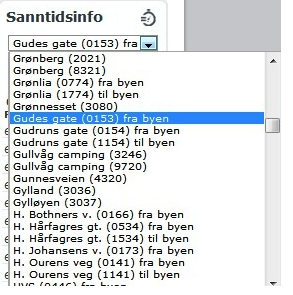
\includegraphics[scale=0.90]{TestingTheApplication/atb2.png}
  \end{center}
\label{fig:gudes}
  \caption{From atb.no: Gudes gate, with wrong direction given}
\label{fig:gudes}
  \end{figure}





\subsection{Finalising Raaum's Application}
Raaum's application has several errors (see Section\ref{sec:testing}), and finalising his application was prioritised before the implementation of new functionalities. 
\begin{figure}[!h]
\begin{center}
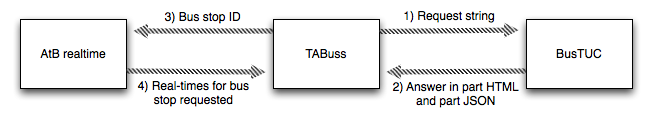
\includegraphics[width=0.9\textwidth]{Method/Figures/noserver.png}
\caption{Query functionality}
\label{fig:noserver}
\end{center}
\end{figure}
\subsubsection{Location}
The user's location is retrieved through a position technology such as WiFi, 3G or GPS. The accuracy depends on the choice, as WiFi provides higher accuracy than 3G. The reason for this, is partially controversial\footnote{http://www.wired.com/threatlevel/2010/05/google-street-view-cams/}: Google scanned and stored MAC-addresses in the process of developing Google Street View. 

Raaum's application has problems displaying the location of the user. The marker used to display the user's location moved when the user zoomed. There is also no indication of how accurate a location fix is. This is solved by the implementation of an Android built-in overlay\footnote{http://code.google.com/intl/no-NO/android/add-ons/google-apis/reference/com/google/android/maps/MyLocationOverlay.html}, where a circle is drawn to display the user's location. The circle's diameter is determined by the accuracy of the location fix. Raaum's application also does not give the user any feedback if a location fix is lost. 

When TABuss starts, it retrieves a location fix and does not proceed until one is present. How long this takes is dependent on location technology, e.g Edge is likely to use more time than WiFi. If the location fix is lost, a warning is given if the user tries to use functionalities dependent on his/her location.

\subsubsection{Map with Bus Stops}
\label{sec:mapsstops}
The displayed map is re-implemented to allow touch events, triggered by pressing bus stop icons. The map is changed to use an ''ItemizedOverlay'' \footnote{http://code.google.com/intl/no-NO/android/add-ons/google-apis/reference/com/google/android/maps/ItemizedOverlay.html}, which the bus stop icons are added to. The XML-file containing bus stop information is also replaced, and TABuss now uses two bus stop lists. One contains information on all bus stops, and one only contains information on one bus stop per bus stop group. The latter is used in the BusTUC query functionality, where only a bus stop's name is required. If we use the list with information on all bus stops, duplicate bus stop names are included in queries. This happens because bus stops within a bus stop group often are located close to each other.

An example of the content in the bus stop lists is shown in table \ref{tab:list}. Each list element contains: The bus stop's ID, the bus stop's name and the bus stop's coordinates.
\begin{table}[h!]
\centering
\caption{Bus stop list}
\label{tab:list}
\begin{tabular}{|c|c|c|}
\hline
 ID & Name & Latitude,longitude \\
\hline
16538544 & \O ie skole &10.254138,63.32273 \\
16011292 & Marcus Thranes vei &10.367198,63.35539 \\
16011374 & Ranheim idrettsplass & 10.521225,63.42812 \\
16010258 & Anders Buens gate &10.429856,63.43846 \\
... & ... & ...\\
\hline 
\end{tabular}
\end{table}

\subsubsection{User Feedback}
An important part of the user experience is to get feedback when errors occur, caused by either faulty user input or a system failure. A system failure in Raaum's application involves errors from BusTUC, the real-time system and the application itself.
In TABuss, feedback is returned to the user both when actions are performed and when exceptions are caught:

\begin{itemize} 
    \item{Progress bars for start-up operations}
    \item{Progress bars for query runs}
    \item{Error message for missing internet connection}
    \item{Error message for missing location fix}
    \item{Error message for missing mounted SD-card}
    \item{Error message for no result found for query}
    \item{Error message for empty input in text fields}
\end{itemize}


\subsection{TABuss}
The following sections provide an overview of the development of TABuss.

\subsubsection{Development Framework}
The development of TABuss has followed Scrum\footnote{www.scrum.org}'s guidelines for iterative development.

\begin{figure}[!h]
\begin{center}
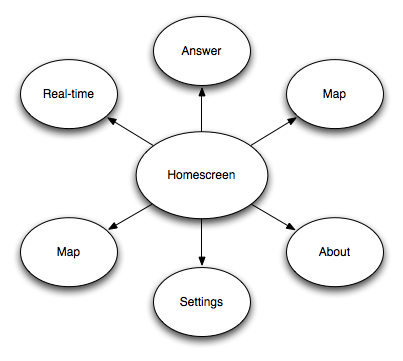
\includegraphics[width = 0.5\textwidth]{Method/Figures/homescreen.png}
\caption{Activity overview}
\label{fig:homescreen}
\end{center}
\end{figure}

\subsubsection{Architecture}
The development part focuses on making usage of the application as easy as possible. By encouraging thumb-navigation, the map is reduced to an extra feature. Raaum's application runs only one activity, which also includes the map. This means map info is downloaded every time the application runs. To avoid this, TABuss is divided into several activities, where the top activity defines a home screen. Menu and button presses start other activities, and the users can choose for themselves whether or not to use the map.

\vspace{0.5cm}
\begin{figure}[ht]
\begin{minipage}[b]{0.5\linewidth}
\centering
\includegraphics[width=0.5\linewidth]{Method/magnus1.png}
\label{fig:figure1}
\end{minipage}
\hspace{0.2cm}
\begin{minipage}[b]{0.5\linewidth}
\centering
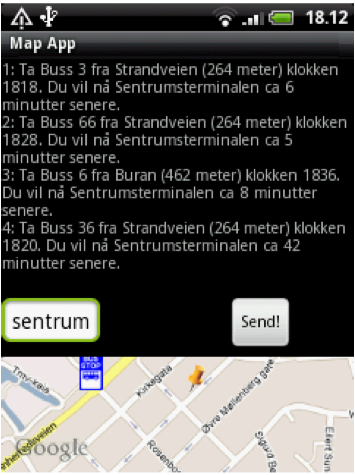
\includegraphics[width=0.5\linewidth]{Method/magnus2.png}
\label{fig:figure2}
\end{minipage}
\caption{Screenshots of Raaum's application.}
\end{figure}

\subsubsection{User Interface}
The user interface in Raaum's application consists only of the screen in Figure \ref{fig:figure1}. Queries are sent and answers displayed in the top section of the screen, while the bottom section displays the map.

One of the most important principles when designing a user interface, is simple and intuitive usage. Extended functionalities require more screens, and has to be solved carefully to achieve user friendliness.

According to \cite{mchallenges}, one of the challenges in mobile computing is the small displays. Even though this article was written in 1994 and the size and resolution of mobile devices have increased since then, it remains a challenge. While a laptop-computer has a 15 inch screen, the minimum requirement for an Android device is 2.5 inches and QVGA resolution (240 $\times$ 320 pixels)\footnote{http://source.android.com/compatibility/index.html}. To cope with the small screen sizes, the amount of elements in the user interface is reduced to a minimum.

\begin{quotation}
\emph{
The acronym KISS (Keep It Simple, Stupid) applies well to interface design. A simple, effective interface should be designed with the users' needs taking first priority.} \cite{guikisses}
\end{quotation}
\vspace{10 pt}
\begin{figure}
\begin{tabular}{ccc}
\includegraphics[width=0.25\linewidth]{DesigningGUI/magnus1.png} & 
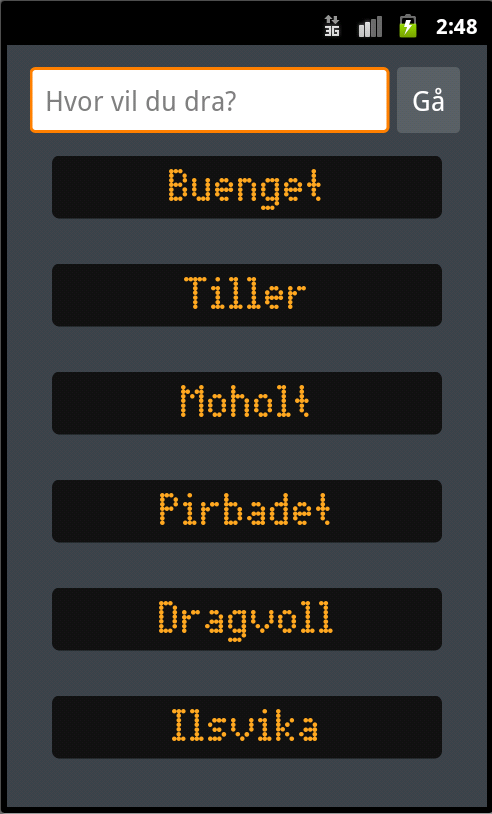
\includegraphics[width=0.25\linewidth]{DesigningGUI/earlydraft.png}&
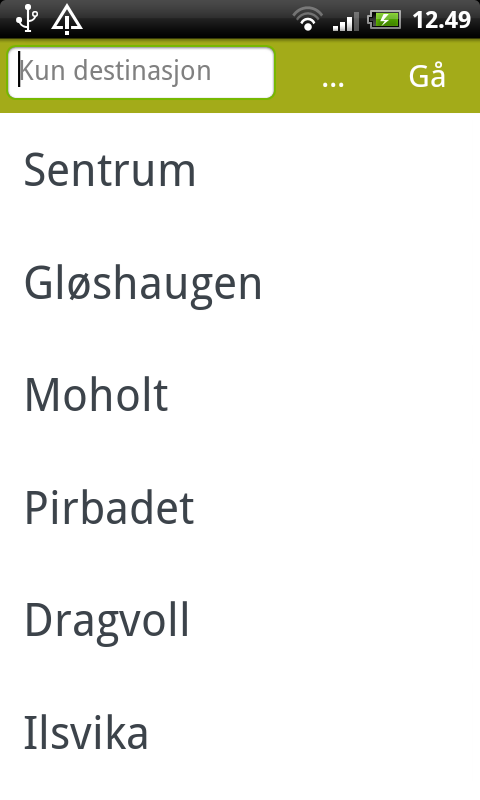
\includegraphics[width=0.25\linewidth]{DesigningGUI/finaldraft.png}
\end{tabular}
\caption{a) Raaum's home screen, b) First draft, c) Final draft}
\end{figure}
The user interface is designed following the ``KISS'' and the ``Less is more'' principles. We want to keep it as basic as possible, while still being aesthetically pleasing. Icons are not used as we want focus on the displayed text.

We chose to use the colours from the AtB website\footnote{www.atb.no}, as these colours are associated with buses by the people in Trondheim.
An early version of the user interface had buttons resembling the LCD signs found on the front of buses, but as the user interface in other features of the application did not have a similar look, a more simplistic approach was chosen in the end. Contrasting colours are used to make the text visible under various lighting conditions.

The route suggestions in Raaum's application are text based. This is not a very good solution for handheld devices with small screens,and is redesigned to show only the most important information, where intuitive layout replaces unnecessary text.

\begin{figure}[!h]
\begin{center}
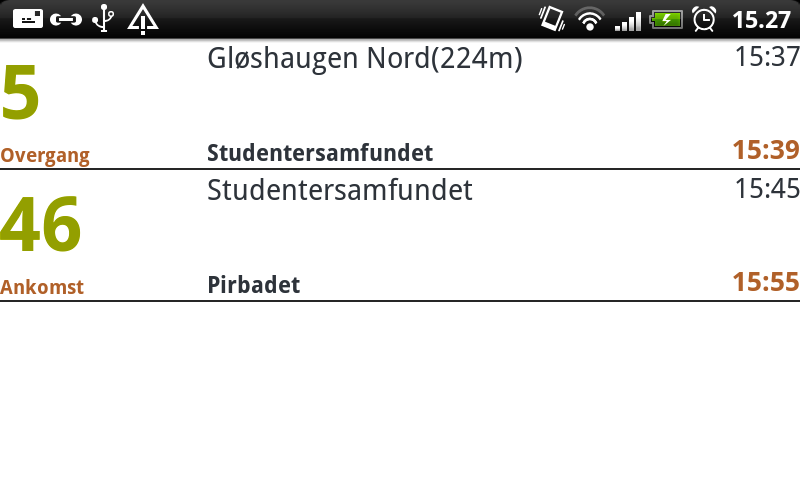
\includegraphics[width=0.5\linewidth]{DesigningGUI/suggestion.png}
\caption{The answer screen.}
\end{center}
\end{figure}

\subsubsection{Context Awareness}
\label{sec:contextawareness}

Context is mainly extracted from the user's location. The device's location listener automatically loads the bus stop objects(from the bus stop list) closest to the user's location, when a location change has been triggered. Real-time data for these can be accessed from the map, or through a list available in the menu. The closest bus stops also play an important part in the main query functionality, where the user's location determines which bus stops are included as departure stops.
\setlength{\intextsep}{0pt}
\begin{wrapfigure}{l}{0.5\textwidth}
  \begin{center}
    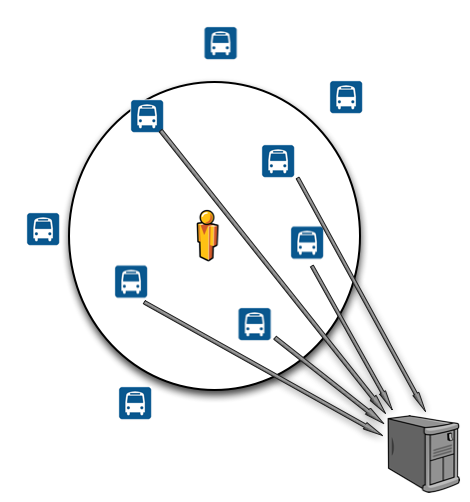
\includegraphics[scale=0.3]{Method/enfigur.png}

  \end{center}
  \caption{Context retrieval}
\end{wrapfigure}
\setlength{\intextsep}{3pt}
To distinguish TABuss from the many existing solutions, extra functionality is added by giving the user the option to let the application guess where he/she is going. A simplified version of case-based reasoning \cite{aam} is implemented, by logging each made query as a case. These data are stored locally in a database, where each case consists of: The departing area, time of day, day of week and destination. Departure areas are squares of 500 $\times$ 500 metres, with defined area codes stored in a separate table. Whenever a new log item is created, a new area is created if the origin location is not covered by an existing area.

To retrieve relevant cases, queries with similar origin and time are fetched from the database. Similarity is implied by identical areas and somewhat similar time of day. For now, +/- 2 hours is used. The retrieved cases are rated by the euclidean distance between each case, and the current time and weekday. The best matching destination is then presented to the user. +/- for hours is used as finding a direct match is difficult. We want to also include delayed bus departures, and bus departures from within a time period.

When TABuss suggests a route, the user can respond by validating the result. At the current moment positive user feedback triggers a query run, while negative feedback has no effect.

The level of intelligence is fairly low, but is still higher than in functionalities with direct look-ups, e.g ''if val.equals(another)''. 

\begin{figure}[!h]
\begin{center}
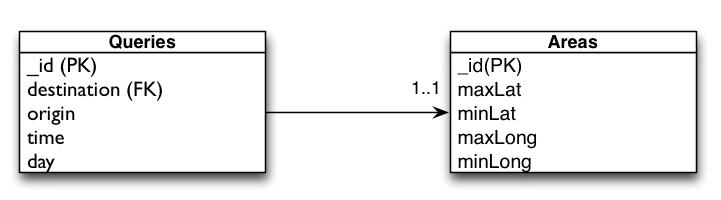
\includegraphics[scale=0.3]{Intelligence/database.png}
\caption{Database tables}
\end{center}
\end{figure}
\newpage
\subsubsection{BusTUC and Natural Language}
To enhance the use of natural language in TABuss, new functionalities which use BusTUC are implemented. Raaum's application only requires a destination as input, which limits the amount of natural language provided to the system. New functionality is firstly the option to switch between the BusTUC syntaxes, defined in section \ref{sec:bustuc}. While the new syntax assumes that the user wants to depart from one of the closest located bus stops, the standard syntax allows for user defined departure stops. Switching between the two BusTUC syntaxes can be done in the home screen menu.

The second part involves AtB's text messaging service\footnote{https://www.atb.no/spoer-bussorakelet/category228.html}. An SMS query starts with ''rute''(route), followed by text, to 2027. This has been incorporated in two ways. If the new BusTUC syntax is chosen from the home screen menu, TABuss uses the closest bus stop to the user's location as the departure stop. If the standard syntax is chosen, the user has to provide both departure and destination input.


\begin{figure}[!h]
\begin{center}
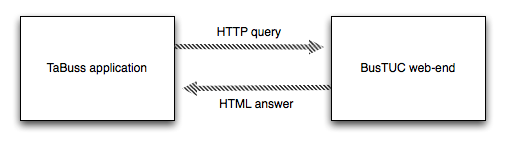
\includegraphics[width = 0.9\textwidth]{Method/Figures/webend.png}
\caption{Web end communication}
\end{center}
\label{fig:webend}
\end{figure}

\begin{figure}[!h]
\begin{center}
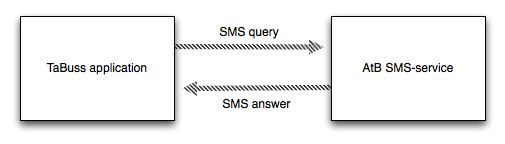
\includegraphics[width = 0.9\textwidth]{Method/Figures/sms.png}
\caption{SMS communication}
\end{center}
\label{fig:sms}
\end{figure}


\subsubsection{Real-time Functionality}
Real-time data can be accessed from the map by pressing a bus stop icon, or through the home screen menu. Both functionalities use the user's location to retrieve and display the $n$ closest bus stops.

The retrieval of a bus stop's ID is done by comparing the chosen bus stop's location with the locations of each of the $n$ closest bus stops. If matched, the found bus stop ID is used to extract the real-time ID. The real-time ID is then sent via SOAP to the real-time server, which returns the five next bus departures.
The user can also search for bus stops that are not among the $n$ closest, by providing a bus stop name as input. This option also lets the user select which direction to retrieve real-time data for(from/towards the city centre), before a real-time query is sent.

\subsubsection{Storage}
The external and internal storages are used with SD-card external storage, and a SQLite\footnote{http://www.sqlite.org/} internal storage database. Favourite strings are stored on the SD-card in text files in a ''favourite'' folder. On application start-up, these are retrieved and displayed in the home screen as query shortcuts. The SD-card also stores a text file with all bus stop names. This list is used for the auto-completion functionality in the input text fields.

The SQLite-database contains logged queries and a history of performed real-time searches for bus stop names. The latter allows quick retrieval of previously performed searches.

\subsubsection{Display of Answers}
The display of query answers is built from scratch. Route suggestions are displayed in a list view, where touch events on a list element trigger a map activity. This map activity shows: The user's location, the location of the selected departure bus stop and a walking route between the two locations. As mentioned in section \ref{sec:maps}, Android does not provide direct access to the Google Maps API, and no native functionality for plotting is available. Our solution is to use KML-files\footnote{http://code.google.com/intl/no-NO/apis/kml/documentation/} for retrieval of walking coordinates between locations. Plotting is done using an ''ItemizedOverlay''.



\subsubsection{Optimisation}
To not the map as a main feature is an optimisation, as data traffic is minimised. Other implemented optimisations are according to the limitations with handheld devices. Unnecessary object creations are avoided by using static calls. Existing objects are also used across \emph{activities} if possible. The application will then check whether or not the needed objects exist, and only create new instances if not. As \emph{activities} over time can ''pop out'' of the \emph{activity stack}\footnote{http://developer.android.com/reference/android/app/Activity.html}, initialised objects do not always exist for the entire application lifetime.

Logical computations are put in \emph{asynchronous threads}\footnote{http://developer.android.com/reference/android/os/AsyncTask.html}. This parallelisation makes the start-up of the application faster, and also allows for progress bars to be integrated. Threading is also introduced in the retrieval of real-time data for route suggestions, where a computation time half of the original is achieved. The application creates a new thread for each bus stop to retrieve real-time data for, and sends all queries in parallel. The threads are stopped and removed by a recursive call, when all queries have returned answers.

\subsubsection{Shifting Functionality to MultiBRIS' Server}
To shift core functionality to a separate server has advantages. During the mentioned Google I/O talks referred to in section \ref{sec:nativeweb}, Reto Meier emphasised the importance of energy conservation in applications because of battery constraints. As back-end computations are shifted to a server, CPU cycles and battery power are saved. Another advantage is the reduced amount of data traffic. In a query involving BusTUC and real-time updates of the departure times, only one query has to be sent to the server. When the application is used stand-alone, a query has to be sent to each.

However, there are disadvantages with the usage of servers. Adding another layer introduces an error source in the communication between the application and the server. BusTUC and the real-time system can be available, but if the server crashes, the application will not receive a response. A server also has to be maintained and updated. 

Advantages and disadvantages are further described by MultiBRIS\cite{multibris}.


\begin{figure}
\begin{center}
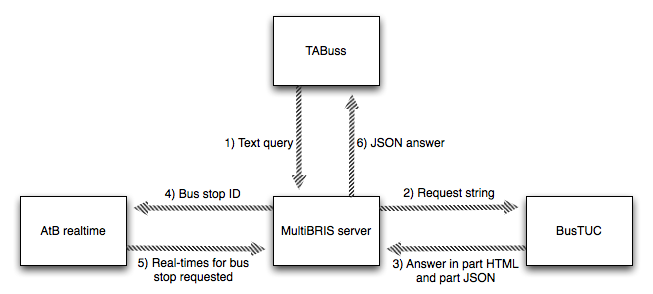
\includegraphics[width = 0.9\textwidth]{Method/Figures/server.png}
\caption{Queries with MultiBRIS' server}
\label{fig:server}
\end{center}
\end{figure}

TABuss benefits from having a modular code architecture, where simple type boolean values control whether to use MultiBRIS' server. Results are either way parsed into dedicated class objects ready for display. 
\newpage

